\documentclass[12pt]{article}

\usepackage[letterpaper, hmargin=0.75in, vmargin=0.75in]{geometry}
\usepackage{float}
\usepackage{hyperref}
\usepackage{graphicx}
\usepackage{url}
\usepackage{copyrightbox}
\usepackage{listings}
\usepackage{csvsimple}

\pagestyle{empty}

\title{ECE 459: Programming for Performance\\Assignment 1}
\author{Zahin Mohammad}
\date{\today}

\begin{document}

\maketitle

\section{Sudoku Solver}
\subsection{Algorithm}
\label{algorithm}
The algorithm used for the sudoku solver is a brute force solution using recursion and back-tracking.
The algorithm will do a \href{https://en.wikipedia.org/wiki/Depth-first_search}{Depth First Search}
for all possible input's for all empty squares.
If the algorithm gets into a state where there are empty squares left on the board, but there are no more possible options,
then the algorithm will traverse back up the call-stack to indicate that that solution path doesn't work, and will try a new input (hence backtracking).
Once a solution is found, the algorithms recurses back up the call-stack to the root caller and returns.
An example of backtracking can be seen in Figure \ref*{fig:back-tracking},
where each "Dead end" is a puzzle with an incorrect solution, and "Succcess!" is a correct solution.
The pseudo code for this algorithim is shown in Listing \ref*{sudoku-solver-pseudo-code}.

\begin{figure}[!h]
    \centering
    \copyrightbox[b]{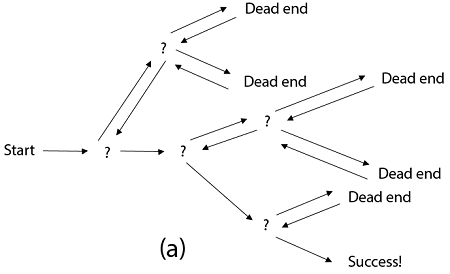
\includegraphics[width=0.6\linewidth]{backtracking-introduction.png}}%
    {Source: \url{https://www.javatpoint.com/backtracking-introduction}}
    \caption{Depth First Search}
    \label{fig:back-tracking}
\end{figure}

\subsection{Possbile Optimizations}
The algorithm described in \ref*{algorithm} is an un-optimized brute force solution. An alternative strategy is to make use of stochastic search techniques such as \href{https://en.wikipedia.org/wiki/Simulated_annealing}{Simulated Annealing} . By introducing a score, or a measure of how "good" a solution is, we can lead the algorithm down a more focused path instead of attempting all solutions. In the case of the sudoku puzzle, a score that can be employed by the simulated annealing algorithm is the sum  of violations in the solution in each row, column and sub-grid, and with this the simulated annealing algorithm would aim to find a solution that minimizes this score. The downside to simulated annealing is the possibility of getting stuck near the end of the search and not resulting in a solution, but the optimization of the optimization will have to be discussed in another report.

\begin{lstlisting}[language=python, caption={Sudoku solver python pseudo code}, label={sudoku-solver-pseudo-code}]
    def solve(puzzle, square) -> bool:
        # Loop all valid sudoku square values, values [1,9]
        for guess in range(1,10):
            # DFS by calling solve with new puzzle
            # Back track to caller if this is the correct solution     
            puzzle[square] = guess
            if solve(puzzle, square.next):
                return True
            # Revert to last valid puzzle state and try next guess
            puzzle[square] = None
            
\end{lstlisting}

\section{Nonblocking I/O}
The provided code to verify the sudoku solutions used synchronous I/O. An optimization to this was to leverage concurrency to verify multiple solutions at the same time. Using "Hyperfine", the different methods can be quantified, and they are explored in subsequent sections.

\subsection{Using Curl Multi}
To achieve concurrency, the \textit{curl multi} crate was used. Using \textit{curl multi}, all the puzzles that are to be verified are registered with \textit{curl multi} and then \textit{curl multi} will verify up to a specified amount of puzzles concurrently. Within this lab, 100 puzzles where set to be verified at a time to reduce the load of the sudoku verifier server. The request response handling is done once all the requests have been finished, and \textit{curl multi} no longer has any requests remaining. The rust code to achieve this is present in file  \url{/src/verify.rs}.

\subsection{Benchmarking Blocking vs Non-Blocking}
During the first benchmarking test, the number of puzzles tested where [1, 10, 100, 200, 300, 400, 500] for both blocking and non-blocking I/O with 100 max connections for the non-blocking case. This test was to highlight the stark difference between non-blocking and blocking I/O. It can be seen in Figure \ref*{fig:Benchmarking} and Table \ref*{table:benchmarking-nonblocking} that Non-Blocking I/O is much more preformat than Blocking I/O, almost by a factor of 86 for the 500 puzzles case. The data used to generate the graph is show in Table \ref*{table:blocking-vs-nonblocking}.

\begin{figure}[!h]
    \centering
    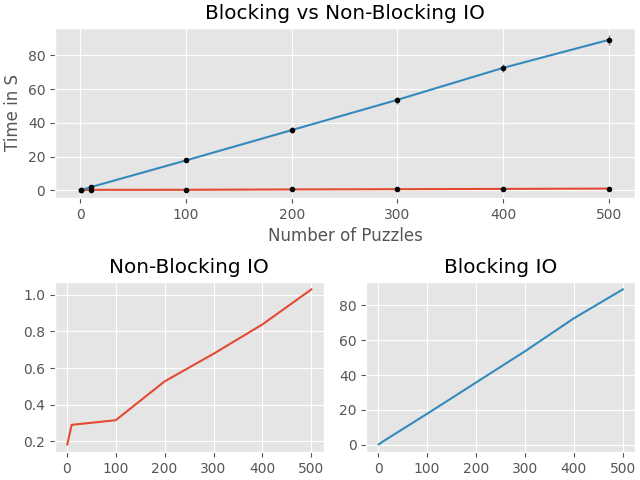
\includegraphics[width=0.6\linewidth]{../plot/graph.png}
    \caption{Benchmarking results for blocking vs non-blocking I/O}
    \label{fig:Benchmarking}
\end{figure}

\begin{table}
    \centering
    \csvautotabular{data.csv}
    \caption{Benchmarking results for blocking vs non-blocking I/O}
    \label{table:blocking-vs-nonblocking}
\end{table}

\subsection{Benchmarking Number of Connections}

During the second benchmarking test, non-blocking I/O was used with a constant 500 puzzles while the number maximum connections configured for \textit{curl multi} where varied with values [3, 4, 16, 32], and this was compared against the blocking I/O case. The results can be viewed in Figure \ref*{fig:benchmarking-nonblocking1} and Table \ref*{table:benchmarking-nonblocking1} (the timing for 500 puzzles for blocking I/O value is seen in Table \ref*{table:blocking-vs-nonblocking}). The results seem as expected. Comparing the case of 16 max connections vs 32 we can see that we see the mean time reduced by half, which correlates to the doubling of the maximum connections.

\begin{figure}[!h]
    \centering
    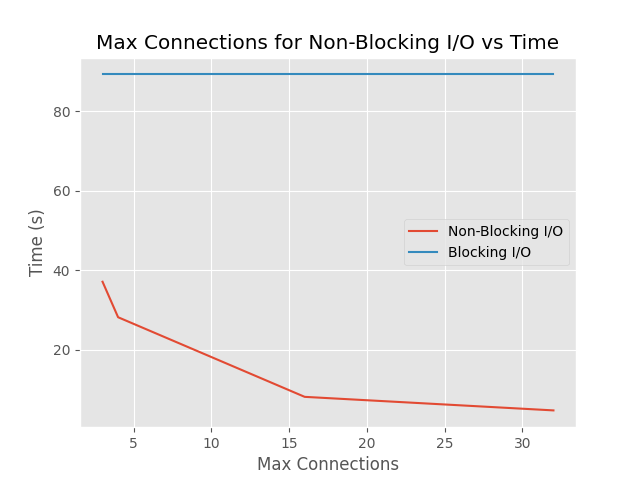
\includegraphics[width=0.6\linewidth]{../plot/num_connections/graph3.png}
    \caption{Benchmarking results for non-blocking I/O}
    \label{fig:benchmarking-nonblocking1}
\end{figure}

\begin{table}
    \centering
    \csvautotabular{data3.csv}
    \caption{Benchmarking results for non-blocking I/O compared}
    \label{table:benchmarking-nonblocking1}
\end{table}








An additional test was performed with just the non-blocking I/O with varying maximum connections between 10 to 100 with increments of 10. The results can be seen in Figure \ref*{fig:benchmarking-nonblocking}, and it is clear that the larger the maximum number of connections, the faster the program finishes. The theory behind this result is that the more connections there are, the more concurrent requests are being made i.e. more network requests per second. It is to be noted that the rate of increase of performance decreases as the number of connections increase. This indicates that after a certain point, there is no additional value in increasing the number of maximum connections. From Figure \ref*{fig:benchmarking-nonblocking}, the point where the rate of change seems to decrease/slow down is around 40-60 maximum connections. 

\begin{figure}[!h]
    \centering
    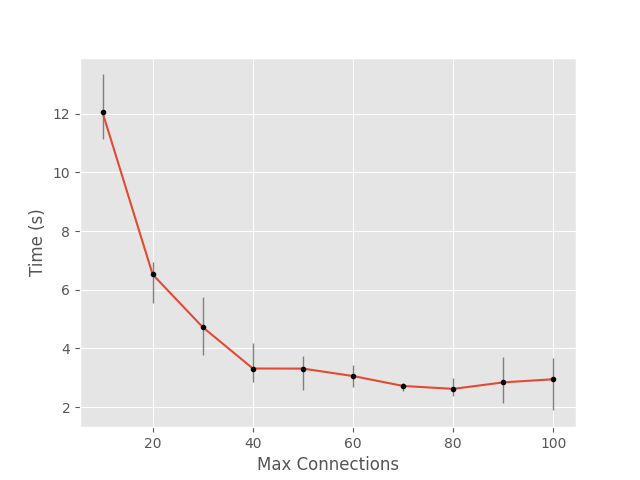
\includegraphics[width=0.6\linewidth]{../plot/num_connections/graph.png}
    \caption{Benchmarking results for non-blocking I/O}
    \label{fig:benchmarking-nonblocking}
\end{figure}

\begin{table}
    \centering
    \csvautotabular{data2.csv}
    \caption{Benchmarking results for non-blocking I/O}
    \label{table:benchmarking-nonblocking}
\end{table}

\end{document}

